% !TEX encoding = UTF-8 Unicode

\documentclass[12pt,a4j,titlepage]{ltjsarticle}
\usepackage{thesis}
\usepackage{listings}
\usepackage{url}
% \title{}
% \author{}
% \date{}

\begin{document}

\begin{titlepage}
  \begin{center}
  
    \vspace*{20truept}
    
    {\LARGE 2024年度 卒業論文} 
    
    \vspace*{75truept}
    
    {\Huge  アメリカザリガニによる水質の
    
    変化についてのシミュレーション} %論文タイトル

    \vspace{10truept}

    {\Huge } %論文タイトル 長い場合 改行1

    \vspace{10truept}

    {\Huge } %論文タイトル 改行2

    \vspace{30truept}
    
    {\LARGE 指導教員 須田 宇宙 准教授}
    
    \vspace{60truept}
    
    {\LARGE 千葉工業大学 情報ネットワーク学科}
    
    \vspace{15truept}
    
    {\LARGE 須田研究室}
    
    \vspace{70truept}
    
    {\LARGE 2132123 氏名 福田 勇太 2132129 氏名 堀田 桃乃介  } % 氏名は消さない 学生番号 氏名 名前

    \vspace{15truept}
  \end{center}
  \begin{flushright}
    {\LARGE 提出日 2025年1月17日}
  \end{flushright}
\end{titlepage}

\setcounter{tocdepth}{3}
\pagenumbering{gobble}
% 目次の出力
\tableofcontents
% 表目次
\listoftables
% 図目次
\listoffigures
\clearpage
\pagenumbering{arabic}
\section{緒言}\label{緒言}
\setcounter{page}{1}
%背景
% 主な淡水魚は, 水草のような水生植物によって浄化された透き通った水環境に生息している.

淡水魚の約25\%は絶滅の危機に陥っている.\cite{FreshWater}
その原因は,水質悪化・遺伝子汚染・乱獲・環境改変など様々な要因があり,淡水魚が生息しづらくなってきている.
中でも,水質悪化が高い割合を占めており,中でも生活排水や外来種によるものがある.
生活排水の関しては,排水規制などにより対処されている事例がある.
外来種の中でもアメリカザリガニによる影響が大きいとされており,水質を浄化している水生植物を切ることで,水質を悪化させている.
また,高い繁殖力と放流により全国各地に生息域を拡大している.

アメリカザリガニの放流を防止させるため,Web,本,学校での授業で啓発活動がされている.
しかし,1,2匹あたりが及ぼす水質悪化の被害の大きさが示されていない.
そのため啓発活動の効果が薄く放流が減らないことが問題である.
1,2匹のアメリカザリガニが与える被害の大きさが具体的に分かれば放流が減り,結果的に水質悪化が抑えられることが期待できる.

そこで本研究では,アメリカザリガニ・水草・水質の相互作用についてのシミュレーションを行うことを目的とする.
\clearpage

\section{淡水魚}\label{淡水魚}
\subsection{淡水魚の生態}
%現在,世界には約35,768種の魚類が存在している.
%うち,約51\%に相当する18075種が,淡水に生息している魚,淡水魚である.
%淡水魚は,清流・濁流・流れの少ない湖など多種多様な環境に生息している.
%しかし,その多くは水草や藻類などの水生植物によって浄化された透き通った水環境を好んでいる.

淡水魚は,地球上の魚類の約40\%を占める重要な生物群であり,世界中の約7,000種が淡水域に生息している.
これらの魚類は,アマゾン流域,アフリカ大地溝帯,東南アジアの熱帯地域,北米の五大湖周辺,そして日本の河川や湖沼など,多様な地理的環境に適応している.\cite{FreshWater}
河川・湖沼・池・湿地帯・小川・渓流といった異なる生息環境において,それぞれの種は独自の生態学的特性を発展させてきた.
水質や温度変化に敏感な淡水魚は,複雑な繁殖戦略と生態系における重要な役割を持ちながら,同時に環境変化に対して脆弱な存在でもある.
淡水魚は人類にとって,単なる生態系の構成要素ではなく,人類の食料供給において極めて重要な役割を果たしている.
特に発展途上国においては,動物性タンパク質の主要な供給源として機能し,年間約2億人の人々の主要な食料源となっている.

\subsection{淡水魚絶滅について}
%近年,生活排水による富栄養化や,外来種が水草などの水生植物を捕食することで起こる水質悪化により,淡水魚が生息しづらくなってきている.
%これにより,淡水魚の約25\%は絶滅の危機に陥っている
淡水魚の絶滅は,現代の生物多様性保全における最も深刻な環境課題の一つとして認識されている.
世界の淡水魚類の約25\%が絶滅の危機に瀕しており,年間約10種が完全に失われつつある現状は,生態系の脆弱性を示している.
この危機的状況は,主に人間の手によってもたらされたものであり,水質悪化・遺伝子汚染・過剰漁獲・環境改変そして外来種の侵入が,淡水生態系に壊滅的な影響を与えている.

\subsubsection{水質悪化}
淡水魚の絶滅における水質悪化は,現代の生態系保全において最も深刻な環境課題の一つとして認識されている.
水質悪化の中でも工業排水・生活排水・外来種によるものが存在している.
外来種による水質悪化は,水中の栄養塩類の循環,溶存酸素量,微生物群集の組成を劇的に変化させ,在来の淡水魚にとって致命的な環境条件を創出している.
また,底質の攪乱,有機物の再懸濁,水の透明度の低下は,淡水魚の生息環境を急速に劣化させ,繁殖,成長,生存の可能性を根本的に減少させている.

工場排水と生活排水は,人間活動に起因する二つの主要な要因により,急速に進行している.

工場排水は,重金属や有機化合物などの有害物質を大量に含み,生態系に壊滅的な影響を与えている.
特に,製造業,鉱業,化学工業から排出される汚染物質は,魚類の呼吸機能を阻害するだけでなく,その生理機能,繁殖能力,免疫システムに深刻な悪影響を及ぼしている.
一方,生活排水は,都市部や農村部から排出される未処理または不十分に処理された排水により,水質環境をさらに悪化させている.家庭からの洗剤・有機廃棄物・栄養塩類などのほか,医薬品の残留物は,水生生態系の基本的な機能を根本的に破壊している.
これらの汚染物質は,水素イオン濃度(pH)の変化・富栄養化・有害藻類の大量発生を引き起こし,淡水魚の生息環境を急速に劣化させている

\subsubsection{遺伝子汚染・遺伝的撹乱}
遺伝的汚染や遺伝的撹乱とは,交雑により遺伝子構造に影響を及ぼし,遺伝子の独自性が損なわれることである.

遺伝子汚染とは,地理的に隔離され,出会うことのなかった近縁種どうしが人為的要因による移動によって出会い交雑し,次世代が形成されることで在来種の遺伝的純系が失われてしまうことである.
原因としては,外来種の侵入や放流や移植である.
遺伝子汚染により,在来種がもつ遺伝的特徴が消失し遺伝子の独自性が失われる.

具体的な例として,タイリクバラタナゴとニッポンバラタナゴの例がある.
タイリクバラタナゴは 1940 年代に中国からソウギョ(Ctenopharyngodon idellus)等の四大家魚に混じり偶然日本に持ち込まれたものである本種は戦後,沖縄県を除く日本全土に分布を拡大した.タイリクバラタナゴの分布の拡大と平行して在来亜種であるニッポンバラタナゴは激減し,本州と四国ではごく一部のため池を除き絶滅したとされている.
タイリクバラタナゴの侵入によるニッポンバラタナゴ絶滅の最大の理由は両者の交雑とされる.
実際,タイリクバラタナゴの侵入によりニッポンバラタナゴが絶滅した生息地の多くは交雑個体が優占する状態となっている[?].

遺伝的撹乱とは長い歴史の中で形成されたある種の遺伝構造や遺伝的多様性が,人為的に持ち込まれた個体との交雑によって乱されることである[?].遺伝子汚染との違いは主に交雑する対象が,異種であるか同種であるかの違いである.
主な原因としては,人為的な放流や移植である.
遺伝的撹乱により,遺伝的多様性の低下であったり.地域特有の環境に適応した遺伝子の喪失により適応能力が低下する.

具体的な例として,アユの例がある.
アユはコイなど漁業権の対象魚種についての増殖義務が課されている.
また,日本の水圏環境が大きく変化する中で失われた自然の再生産を補助する目的で稚魚の放流等が行われいている.
しかし,稚魚の放流により遺伝的に違う両親が交配すると,子孫が弱くなってしまうことや病気になりやすい.
そして最終的には,数が減ってしまう可能性がある.

 \subsubsection{乱獲}
商業漁業,生計手段としての漁業,そして違法漁業による無秩序な捕獲により,多くの淡水魚類の個体数が急速に減少している.
具体的な例として,ウナギはこの問題を象徴する魚種の一つである.
需要の高まりによって,資源量が危機的な水準にまで減少しているためである.
伝統的な食文化と経済的価値が,この種の存続を危うくしている.
乱獲の影響は,直接的な個体数の減少にとどまらず,捕食と被食の関係,生態学的なバランス,遺伝的多様性など,これらすべてが深刻な影響を受けている.
% 特定の魚種の減少にとどまらず,水圏生態系全体の構造的崩壊をもたらす.

\subsubsection{環境改変}
 日本の河川や水域生態系は,人間の開発行為による急速な環境改変により,多くの淡水魚が住処を失う危機に瀕している.
特に河川改修や土地開発によるものがあげられる.
まず河川改修は農業や工業に利用する淡水の過剰な取水により,水路の流れを単調なものに変えたり,コンクリートの護岸の設置などが行われていることである.

土地開発はダムなどの大規模なインフラ開発が主な原因である.
そうすることで,河川や地下水の枯渇を招き,淡水魚の自然な住処を奪い,彼らの移動と繁殖を著しく制限してしまっている.
これらの環境改変の影響は,互いに絡み合い,淡水魚の絶滅リスクを加速度的に高めている.個体数の減少は,遺伝的多様性の喪失につながり,種の存続をさらに危うくしている.
\clearpage

\section{外来種}
\subsection{外来種について}
 本来その地域に生息していなかった生物が、人為的な活動によって意図的または非意図的に新たな環境に持ち込まれ定着してしまった生物種のこと外来種という.
 中でも「特定外来生物」に指定されている種があり,生態系・人の身体・生命・農林水産業へ被害を及ぼすもの又は及ぼすおそれのあるもののことである.
特定外来生物は,新しい環境で天敵が少ないため,急速に繁殖し,爆発的に個体数を増やす傾向がある.
そのため,本来その環境に存在しない捕食者であり,競争相手であるため,生態系のバランスを破壊してしまう可能性がある.

\subsection{被害}
\subsubsection{生態的影響}
外来種がもたらす生態的影響は主に,食害である.
在来の淡水魚の卵や幼体を捕食し,個体数を激減させている.
また,一部の外来種は魚だけでなく水草を切断,また食べることに生態系に影響を及ぼしている.

日本では長い年月をかけて,ナマズやハス,サクラマスなどの肉食魚を頂点とした水圏生態系が成立し,餌となる小型のコイ科魚種などとの微妙な個体数のバランスを保ってきた.
しかし,国外外来魚であるブラックバス類やマス類の導入などにより,生態的地位が同等なナマズやハス,サクラマスなどは,場の占有餌の競合の形で影響を受ける.また,上述の国外外来魚から在来魚が受ける直接捕食により,在来魚の個体数減少や絶滅が生じている.

生態的影響をもたらす外来種の例として,ブラックバスとブルーギルを挙げる.
ブラックバスやブルーギルはオスが産卵床という巣をつくり,そこにメスを誘って産卵する.そして産んだ卵は.オスが他の魚から守る.
これは卵がふ化した後,仔魚になってもしばらく続く.
このことは,成魚にまで生き残る確率が高く,増えやすいことにつながる.
ブラックバスは肉食性で自分の体の半分くらいの長さの魚まで食べることができる.
50cm程まで成長するブラックバスに比べて,在来魚はコイやフナなどの一部を除くと小型だ.つまり,大型のコイやフナ以外はみんな餌になってしまう.
またブルーギルは雑食性で,魚の卵が好物である.産んだ卵を守るブラックバスやブルーギルと違って在来魚は卵を産みっぱなしにする種類が多く,
卵がブルーギルに食べられてしまう.

\subsubsection{遺伝的影響}
在来種は近縁な外来種と交雑することがよく知らている.
また,近縁な外来種と交雑することで起こる被害が遺伝子汚染や遺伝的撹乱と呼ばれている.
遺伝子汚染とは,地理的に隔離され,出会うことのなかった近縁種どうしが人為的要因による移動によって出会い交雑し,
次世代が形成されることで在来種の遺伝的純系が失われてしまうことである[?].
次に,遺伝的撹乱とは長い歴史の中で形成されたある種の遺伝構造や遺伝的多様性が,人為的に持ち込まれた個体との交雑によって乱されることである[?].
遺伝子汚染との違いは主に交雑する対象が,異種であるか同種であるかの違いである.
また,それほど近縁でない外来魚と在来魚の交雑個体の多くのオスは,遺伝子や染色体の不整合が原因で繁殖能力のないオスとなる.
これらの個体が繁殖行動に加わると,在来種の繁殖率は低下することになる.
このほか,異なる適応度を持つ集団との混合による集団全体の適応力の低下である.
適応度の減退や,交雑による繁殖力の低下などが遺伝的影響として挙げられる.
\subsubsection{病原的影響}
病原的影響とは外来魚有する病原菌や寄生虫が,放たれた先で無抵抗の在来魚へ水平感染し,在来の集団を脅かす影響である.
具体的な例として,冷水病という日本ではアユが大きな被害を受けている細菌である.
冷水病は全国的に大きな問題になっており,この細菌によって天然河川や養殖場でアユが大量に死ぬ事態が起きている.
冷水病菌は魚の肉を溶かして食べてしまう.発病した魚は体表面に穴が開いたり,尾ビレやアゴが欠損したりして死に至る.
また,予防法がないのが現状である[?].
\subsubsection{未知の影響}
外来魚は,移殖先において予測不可能な未知の影響を潜在的に有しており,これはフランケンシュタイン効果と呼ばれる.複雑・精密に構成された在来生態系に対し,影響が被害となって顕在化するまでに時間を要することも多い.分子生物学が未発達であった時代における外来魚の放流が,現在における遺伝的な汚染として顕在化したことについて,当時としては未知の影響であったと想像される.このように,外来魚が在来生態系に及ぼす影響としては,現時点では想定できない未知の影響を潜在的に有していると考えられる[?].
\subsection{アメリカザリガニ}
\subsubsection{アメリカザリガニの生態}
外来種の中で代表的な生物であるアメリカザリガニは,ウシガエルの餌として利用する目的で日本国内に輸入された.
アメリカザリガニの生態的特徴は主に,非常に高い繁殖力・生息可能な環境・雑食性の3つがあげられる.
1年に2,3回の繁殖を行い,1回の産卵で200\textasciitilde1000個の卵を産むことが出来,環境適応力も高く,過酷な環境下でも生存が可能である.
生存環境は水田・池・小川・湿地など様々な水域を好み,水質や温度の変化に耐性が強いため,0\textasciitilde35℃の広い温度の範囲で生存が可能.
摂食行動の面では,雑食性で,水生植物・淡水の小魚・昆虫の幼虫・プランクトン・魚などの死骸とあらゆるものを捕食する.

\subsubsection{アメリカザリガニによる実害の事例}
環境省によると,アメリカザリガニによる水質の悪化が問題視されている.
アメリカザリガニは,底泥を巻き上げる行動や水生植物の切断・食害により,水質を悪化させている.
そのため現在は,条件付特定外来生物に指定されている. 

茨城県の宍塚大池の事例では,2020年ごろにアメリカザリガニが大量発生した.
これにより,水草が著しく減少し,池の水が濁った.
原因としては,以下のような現象が生じたためである.
①図1(左)は水草が生い茂っており,栄養素が過剰にならないようにバランスを保っている\\
②アメリカザリガニにより水草が減少し,富栄養化になる\\
③藻類が栄養素を吸収し異常増殖する.\\
④酸素が不足し,藻類が死滅して水質が悪化し図1(右)のように水が濁る
現在,地域の協力によって1万匹以上のアメリカザリガニが駆除されているが,その繁殖力の強さから完全な駆除には至っていない

\begin{figure}[h]
\begin{center}
  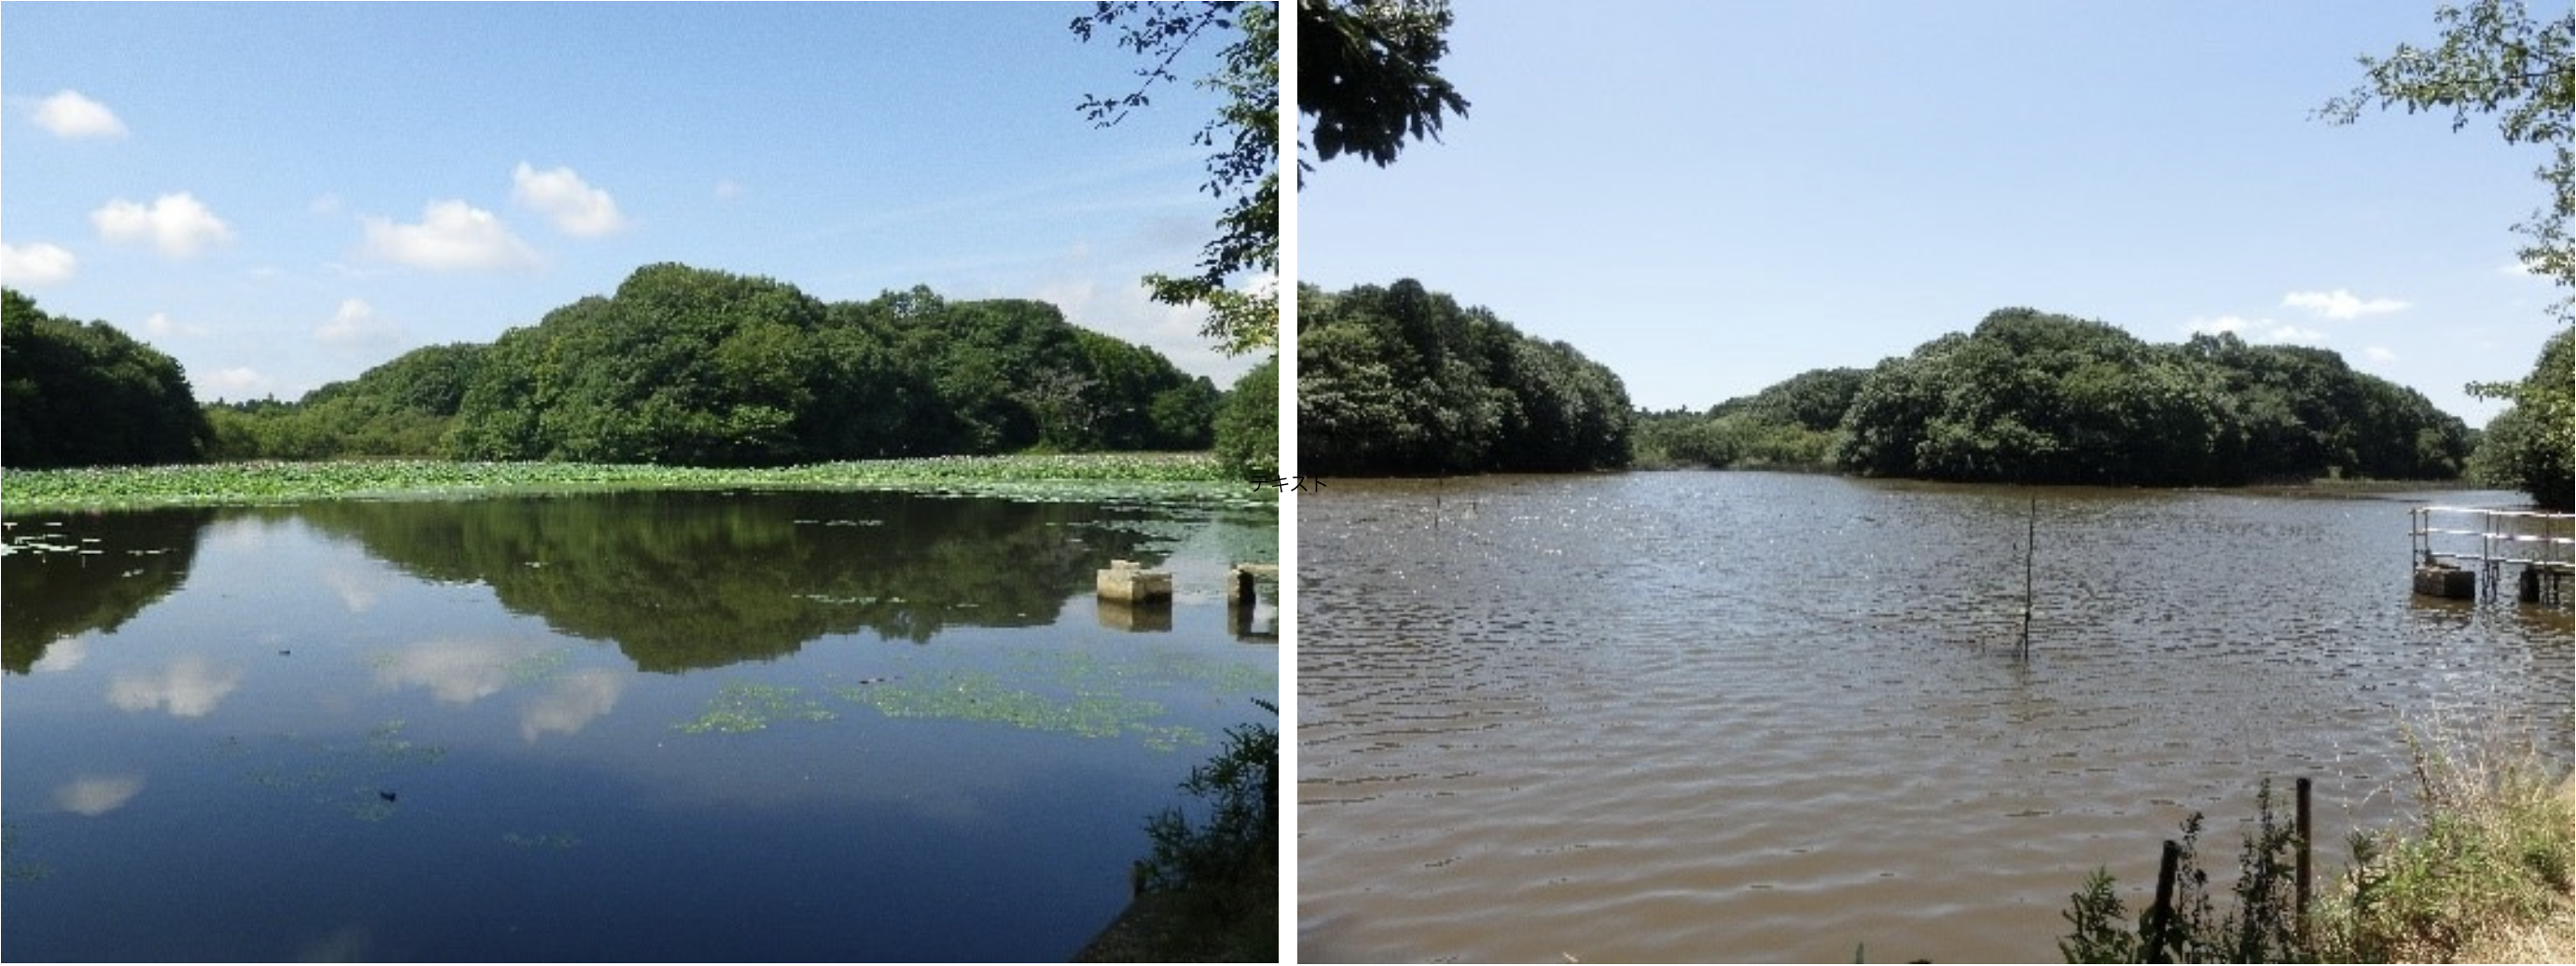
\includegraphics[width=.95\columnwidth]{新・水質.jpg}
\end{center}
  \caption{アメリカザリガニによる影響\\(左:侵入前,右:侵入後)}
  \label{fig:切り替え}
\end{figure}

\subsubsection{今ある啓発活動}

\clearpage
\section{シミュレーションについて}

\subsection{先行研究}

\subsection{生態系モデル}
初めに生態系とは,食物連鎖などの生物間の相互関係と,それをとりまく環境の間の関係をとらえた生物社会のまとまりのことを示す概念である.
次に,生態系モデルとは生物の振る舞いや相互関係の一つ一つを数式で表すことである.
また,表した数式を解くことでコンピュータの中に生態系を再現しシミュレートすることができる.
しかし,生態系には膨大な種類と数の生物が棲んでおり,お互いに影響を及ぼし合っているため,計算は容易ではない.
また,光や温度などの環境も,場所ごとに異なるうえに時々刻々と変化するため,計算は非常に複雑になる.
そして,何より生態系には物理学の運動方程式のような普遍的で厳密な数式が見つかっていない.
そのため,実際にある観測データや実験データから数式にすることや簡単化した方法で計算している.
このようなモデルを作成する目的は生態系のバイオマスの変化や,成長や衰退などをシミュレートすることにある.

生態系の全てをモデル化することは不可能と言っても過言ではないが,特定の要素に絞ることで
シミュレートすることは可能である.
生態学で用いられる古典的なモデルに「ロジスティック方程式」というものがある.
このモデルは,ある単一種の生物が一定環境内で増殖するようなときに,その生物の個体数の変動を予測することできるモデルである
生物は指数関数的に増加する.
しかし,実際には環境や資源は限られているため,生物が増えるに連れて増加率は低減し,生物の増加はどこかで飽和すると考えられる.
ロジスティック方程式は元々存在していた個体数を予測するモデルにこの点を取り入れて,生物の個体数増殖をモデル化したものである.


\subsection{概要}
\subsubsection{アメリカザリガニの繁殖モデル}
本研究では,アメリカザリガニの繁殖をシミュレーションするために式\eqref{eq:one}においてロジスティック方程式を用いる.
この方程式は,生物の増加モデルとして用いられ,単純な指数関数的増加に加え,環境収容力という要素を組み込むことで,生物の個体数が増加するにつれて成長率が低下し,最終的に飽和状態に達することを再現できる.\cite{log}.
N(t)は月における個体数,rは繁殖率,Kは環境収容力である.

\begin{equation}
  N(t+1) = N(t) + \mathrm{r} \cdot N(t) \cdot \left(1 - \frac{N(t)}{\mathrm{E}}\right)\label{eq:one}
\end{equation}
今回シミュレーションを行う期間は40ヶ月と設定した.この期間は, アメリカザリガニによる被害が観察される期間として文献に記載されていた2~3年という期間を参考にし,余裕を持って設定した期間である.
また, 繁殖率rは0.7に設定した.この値は, 水草の減少量が実際の観察データと一致するように調整したものである. アメリカザリガニが条件付き特定外来生物に該当するため, 繁殖率に関する直接的なデータが存在しないので, 複数の候補値を用いてシミュレーションを実行し, 最終的に最も現実の被害量と一致した値を採用した.さらに、環境収容力Kは300,000匹に設定した.
この値は,実験データから導出された1㎡あたりの収容力9匹を池の総面積33,000㎡に適用して算出したものである.具体的には,関連研究において高バイオマス状態が観察された条件を基に計算し,実害の観測地である池全体に拡張する形で設定した.
今回の場合は,実害の観測値は茨城県土浦市宍塚にある宍塚大池である.
この環境収容力の値は,生態系におけるアメリカザリガニの密度上限を表し,モデルにおける増加の抑制要因として重要な役割を果たす.このように設定されたパラメータを基に,アメリカザリガニの個体数変動をシミュレーションする.
シミュレーションの結果が以下である.

 {\begin{figure}[h]
 \begin{center}
   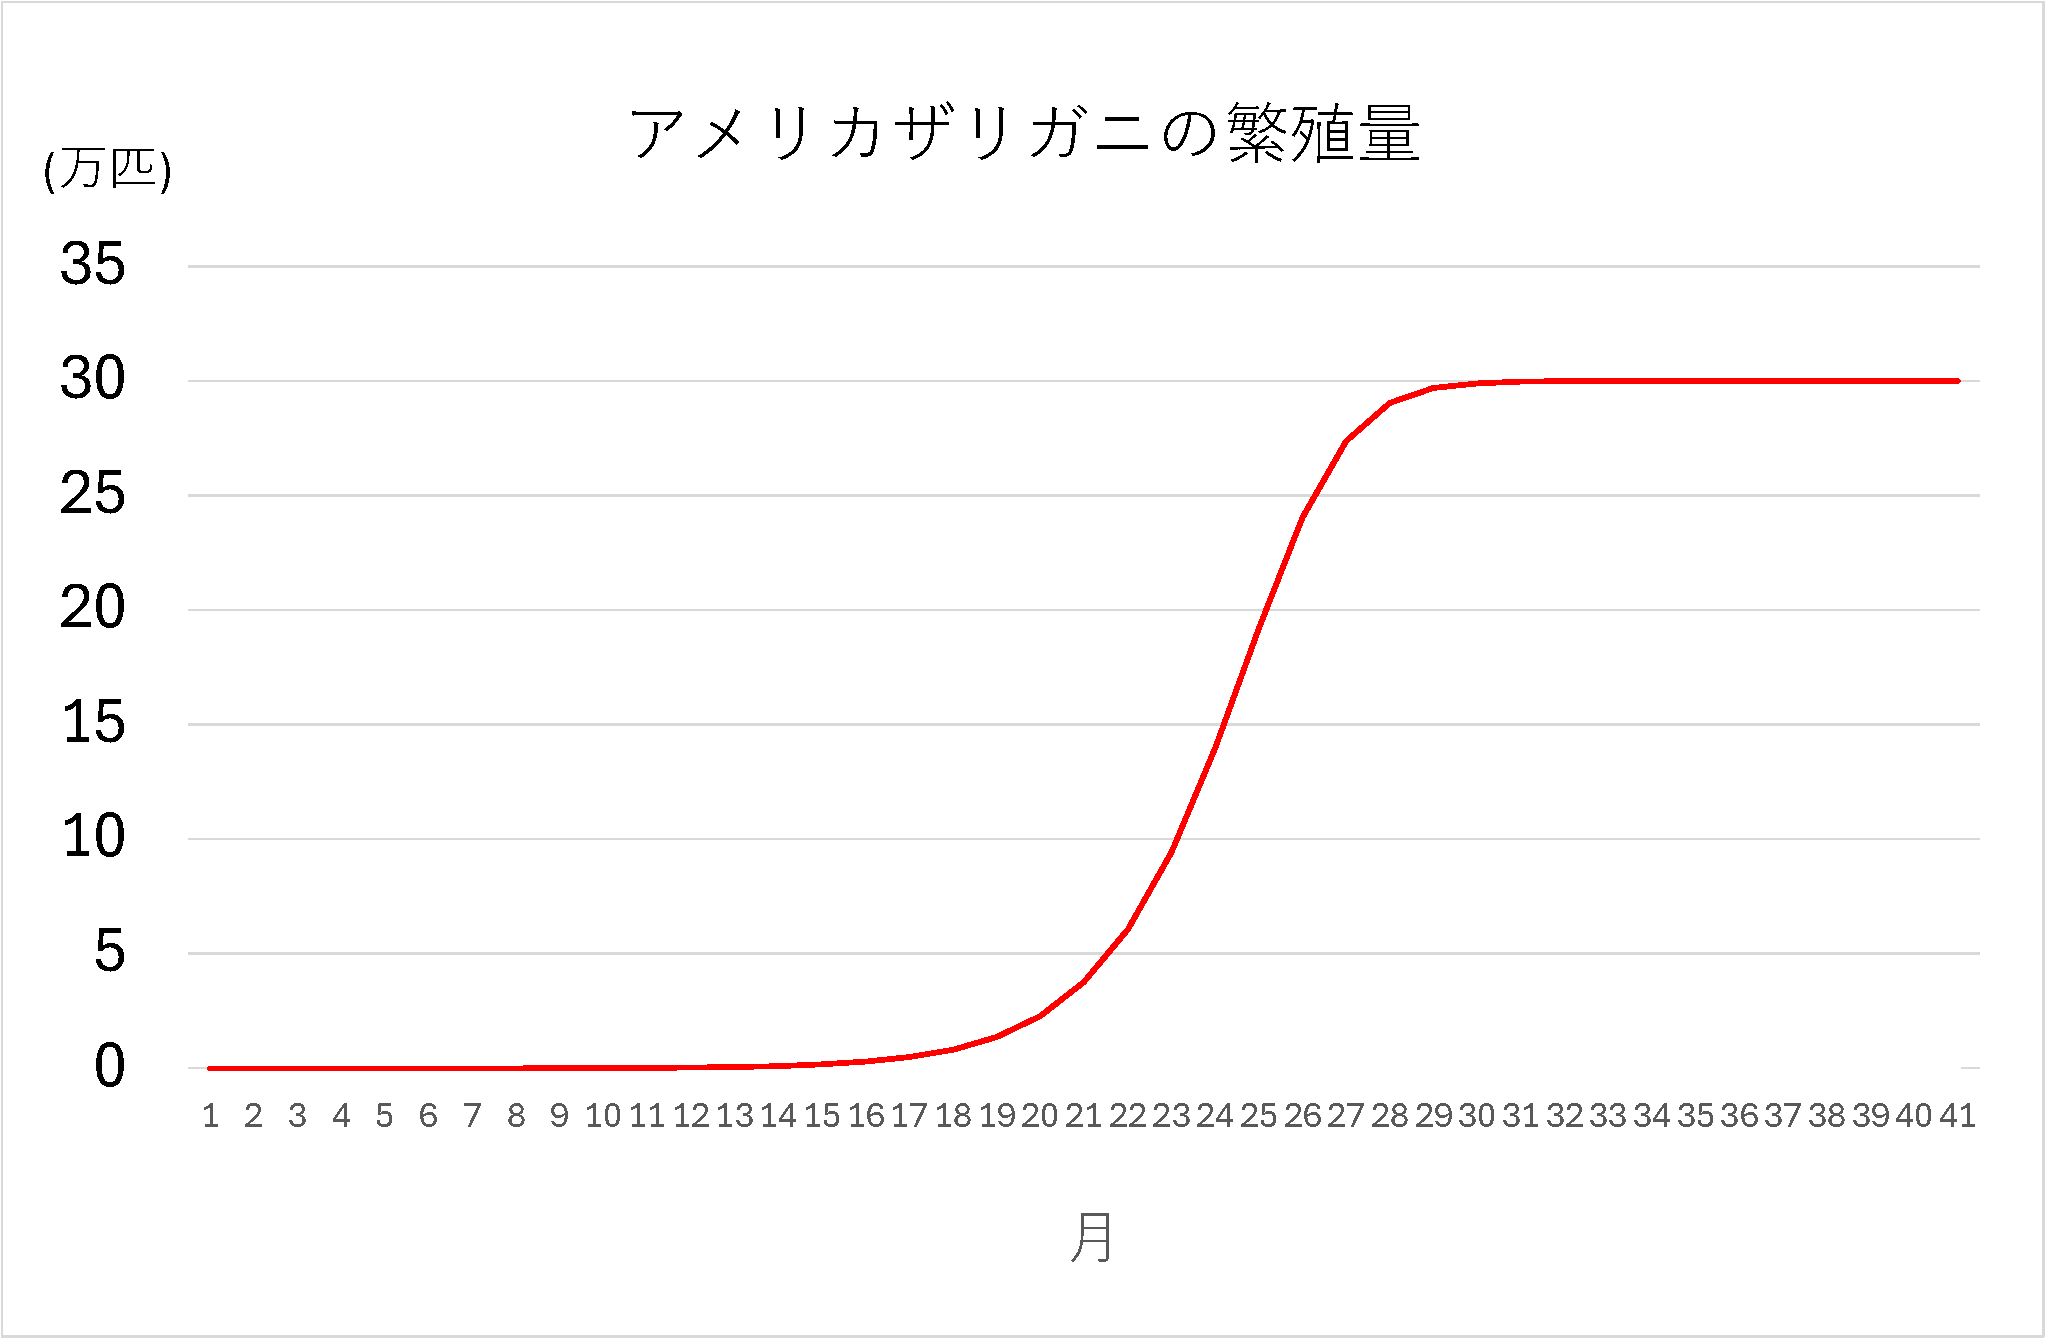
\includegraphics[width=.95\columnwidth]{amezari_graph.pdf}
 \end{center}
 \end{figure}

 図??から,17,18ヶ月ごろから変化が大きくなり始めており,30ヶ月ごろには高バイオマスと言える 30万匹に近づいており,飽和状態になっていることがわかる.
また,アメリカザリガニの急激な繁殖力を表している.

\newpage
\subsubsection{アメリカザリガニによる水草の減少モデル}
アメリカザリガニの繁殖のモデルをもとに作成した水草の減少モデルを式\eqref{eq:two}に示す.具体的には,アメリカザリガニの繁殖の量に応じて水草が減少するモデルである.
$W(t)$はその月における水草の重さ,aは1匹のアメリカザリガニが1ヶ月で減少させる水草の量である.

\begin{equation}
  W(t+1) = W(t) - a \cdot N(t)\label{eq:two}
\end{equation}

今回,シミュレーションを行うにあたってa[g]を80gに設定した.
この値は関連研究において,アメリカザリガニ1匹が1ヶ月で80gの水草を食べるという実験データに基づいたものである.
$W(t)$の初期値として19,305,000[g]に設定した.
この値は関連研究から以下のように計算したものである.

関連研究でのアメリカザリガニの生息環境から水草の総重量を1㎡あたり585gとし,宍塚大池の面積が33,000㎡であることから,以下のように計算した.\\
W(0) = 585 \cdot 33,000 = 19,305,000 \, \text{g}\\
このように設定されたパラメータを基に,水草の変動をシミュレーションする.
シミュレーションの結果が以下である.
また,図?がシミュレーション結果である.

{\begin{figure}[h]
 \begin{center}
   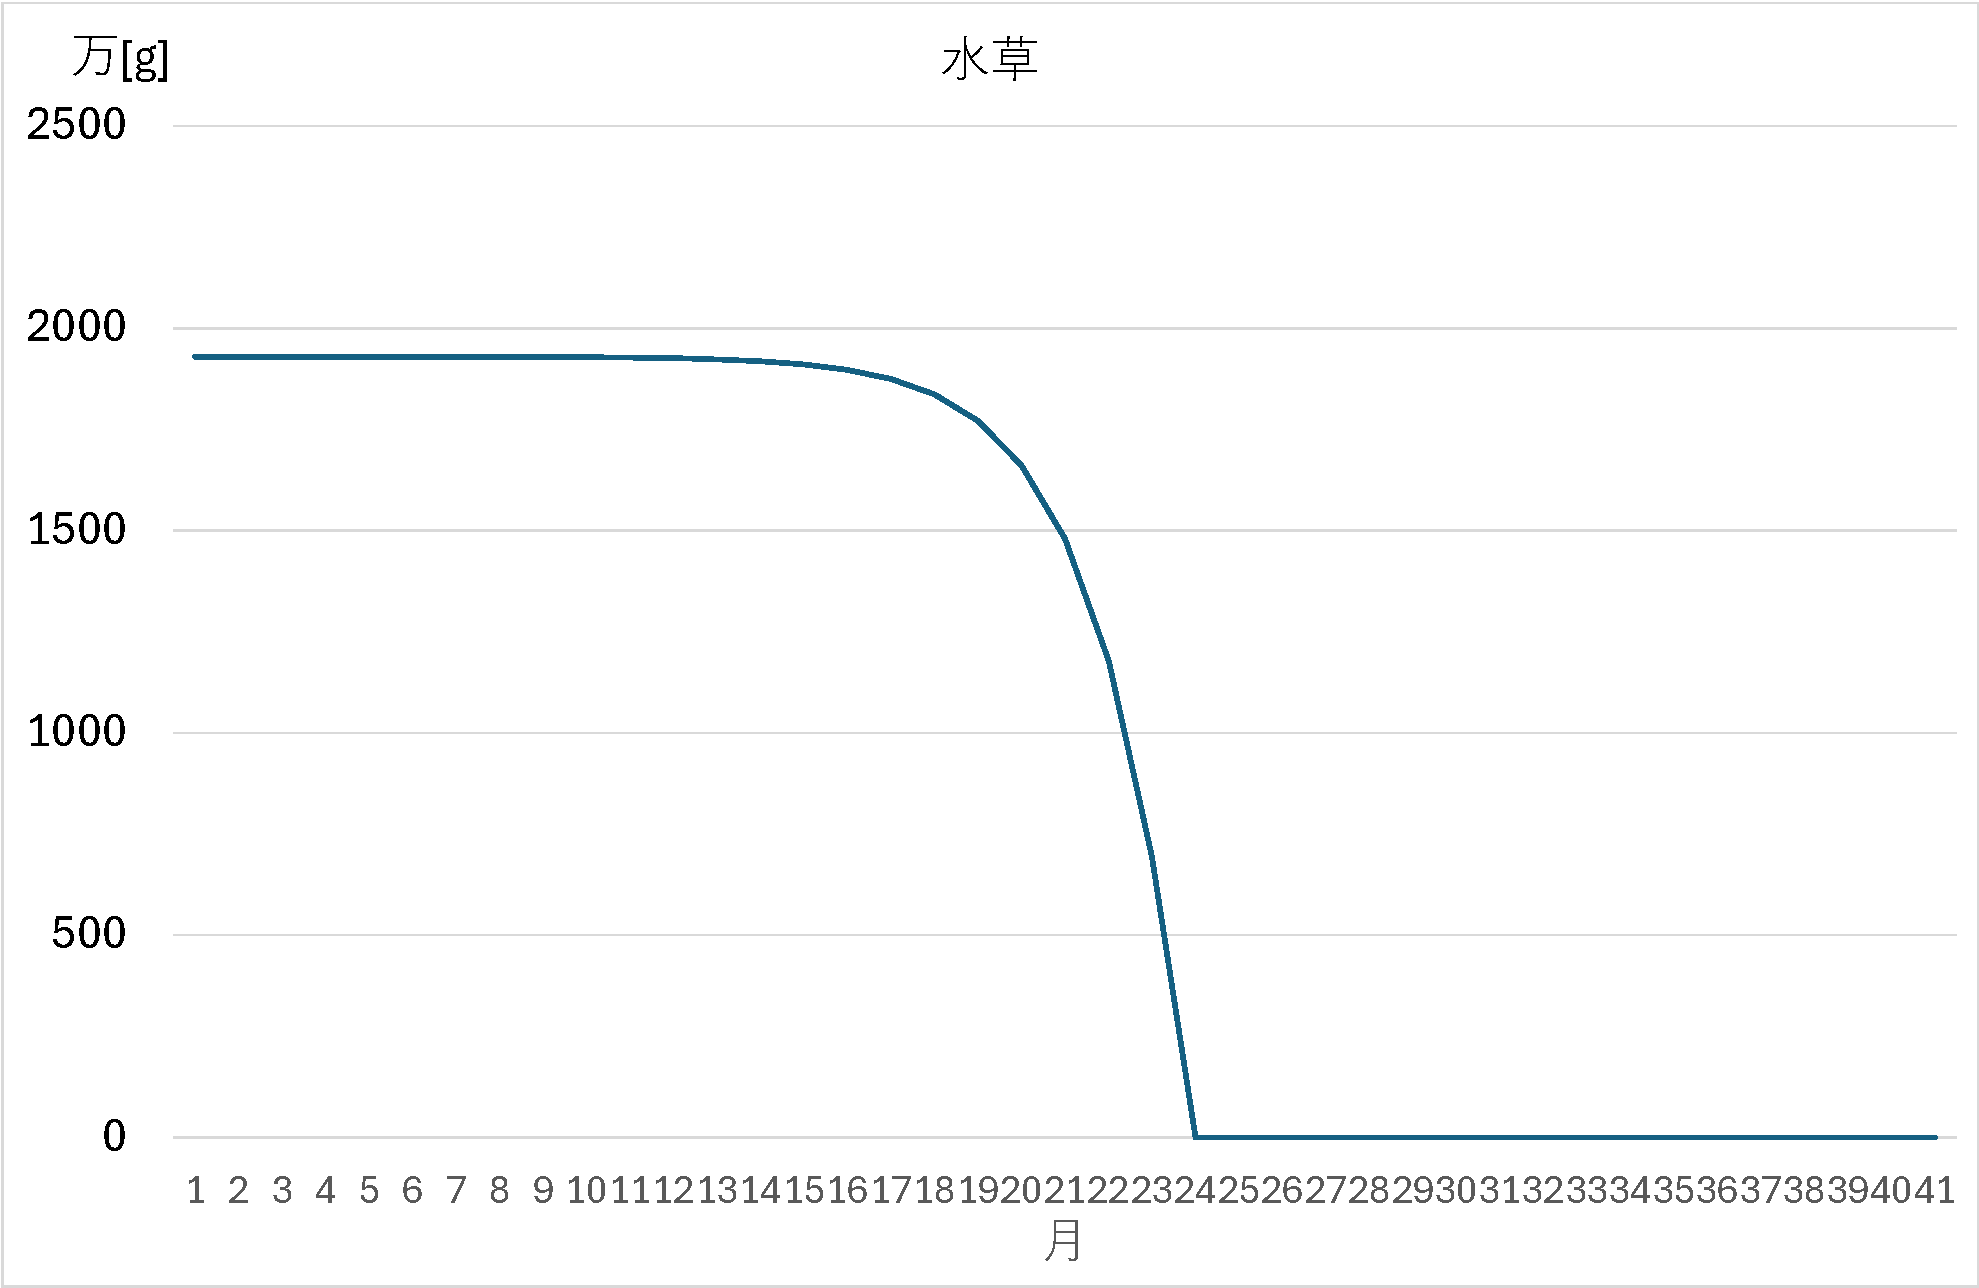
\includegraphics[width=.95\columnwidth]{mizukusa_graph.pdf}
 \end{center}
 \end{figure}
\subsubsection{アメリカザリガニによる水質悪化のモデル}
水草の減少モデルと同様にアメリカザリガニの繁殖モデルをもとに作成した水質のモデルを
式\eqref{eq:three},式\eqref{eq:four}に表す.
水質に関する指標は多数存在するのだが本研究ではSSとクロロフィルa濃度を用いた.
$S(t)$,$C(t)$はその月におけるSS,クロロフィルaの重さ,
$k$,$h$は1匹のアメリカザリガニが1ヶ月で増加させるSS,クロロフィルaの重さ.
Lは水量を表す.

\begin{equation}
  S(t+1) = \frac{S(t) + k \cdot N(t)}{L}\label{eq:three}
\end{equation}

\begin{equation}
  C(t+1) = \frac{C(t) + h \cdot N(t)}{L}\label{eq:four}
\end{equation}

SS(Suspended Solids:懸濁汚染物質)とは,水の濁り,透明度等の外観に大きな影響を与える物質である.
また,アメリカザリガニが底泥を巻き上げる行為によりこの値が増加する.
SSが生態系に与える影響には,魚類のエラを塞ぎ,呼吸を妨げて窒息死させる危険性や,太陽光線の透過 を妨げ,藻類の光合成を阻害させる等がある.さらに,沈降したSSは,底生生物を埋没させて死滅させ,堆積したSSは,二次的汚染を引き起こす。

クロロフィルa濃度とは
水の濁りと植物プランクトンや藻類に含まれる光合成色素である.
光合成色素とは光合成において光エネルギーを吸収するための色素である.
濃度が高いと植物プランクトンや藻類の増殖が予想できる.
これはアメリカザリガニが水草を切断・食害により異常増殖する.

また,図?がシミュレーション結果である.

{\begin{figure}[h]
 \begin{center}
   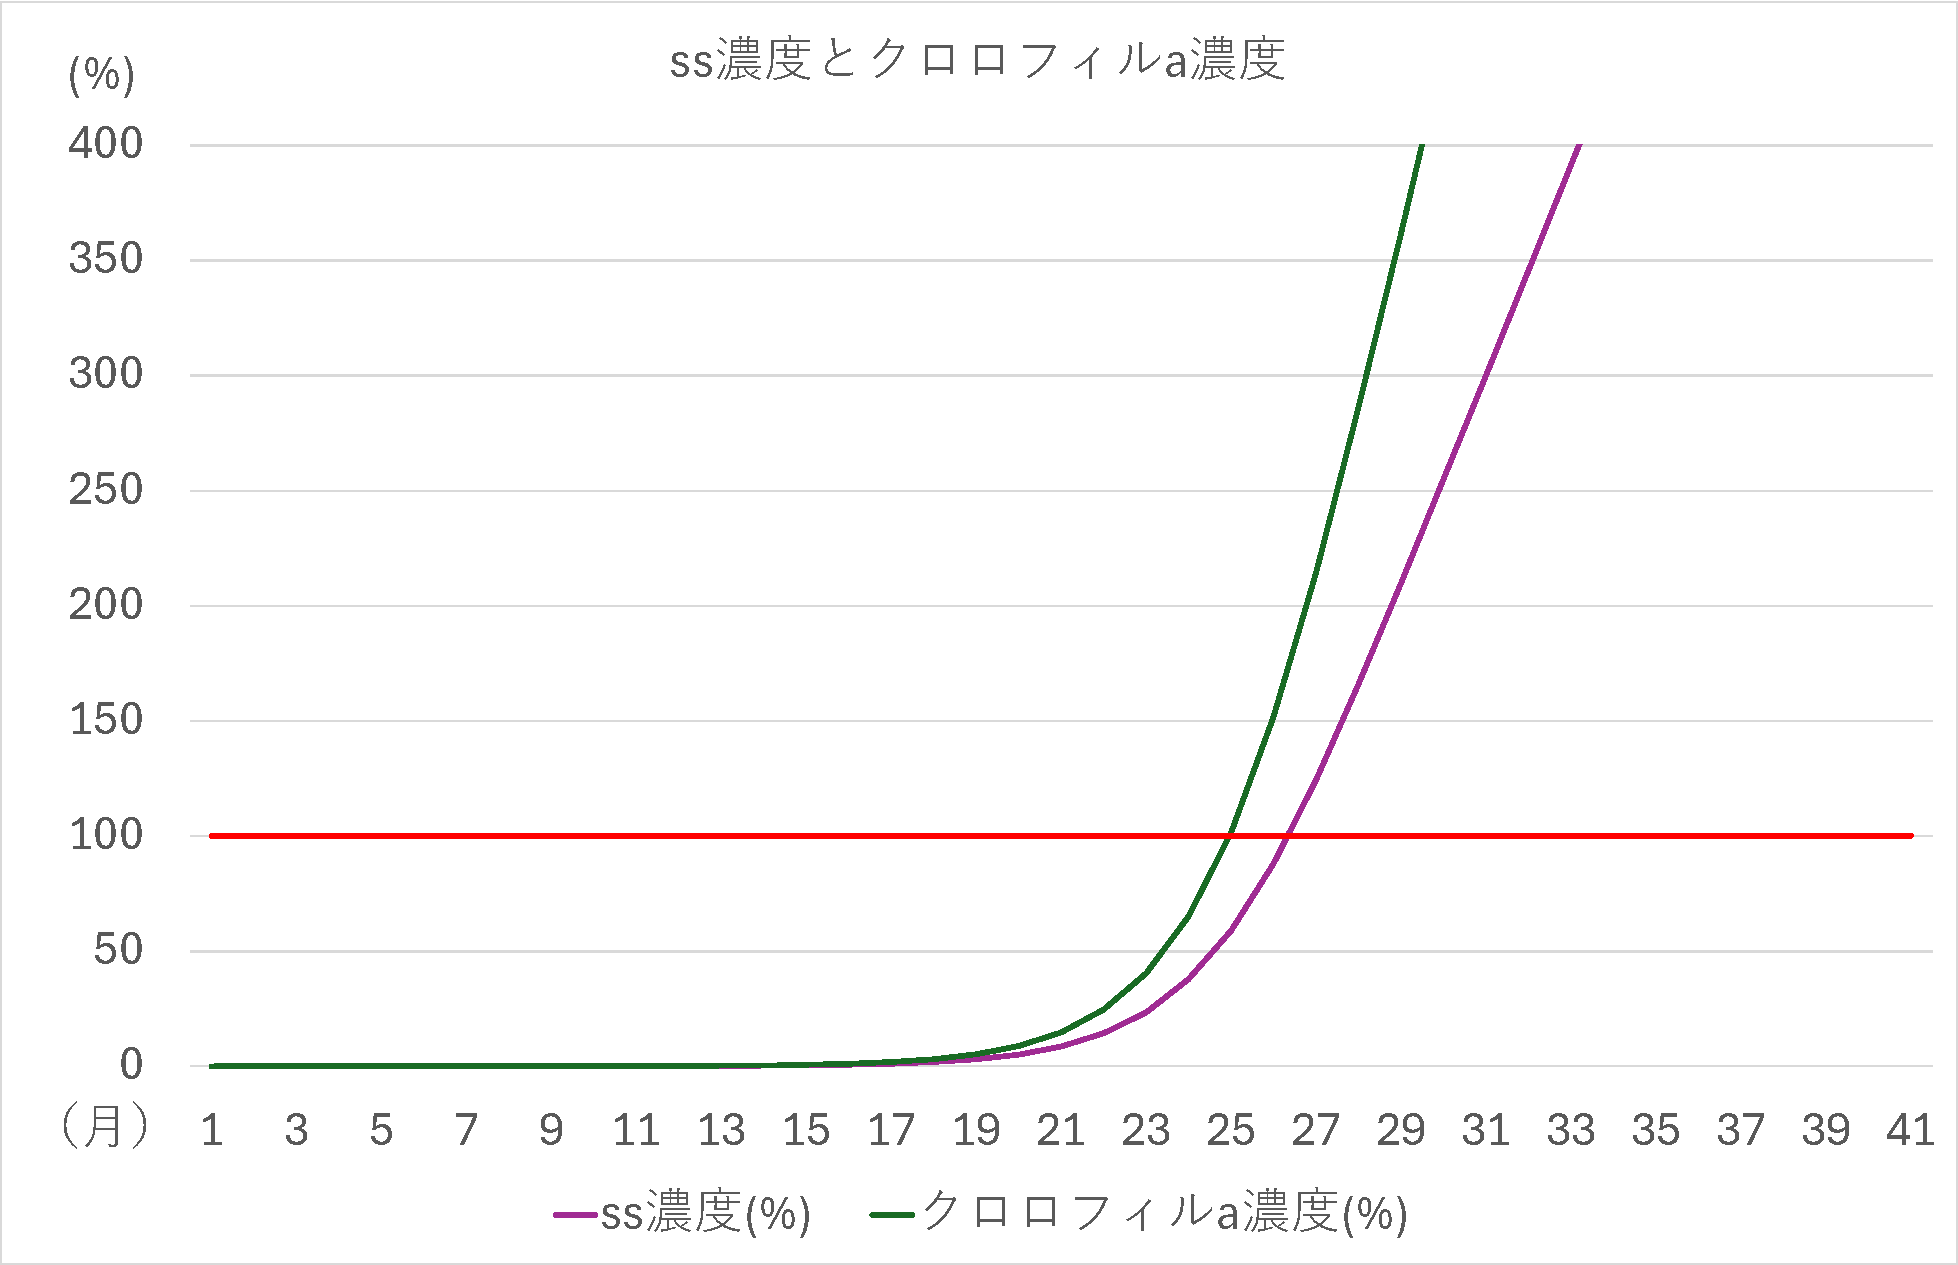
\includegraphics[width=.95\columnwidth]{SS_Chl_graph.pdf}
 \end{center}
 \end{figure}

\newpage
\subsection{シミュレーション結果}
今回作成したアメリカザリガニの繁殖モデル,水草の減少モデル,水質のモデルを図??に
示す.
{\begin{figure}[h]
 \begin{center}
   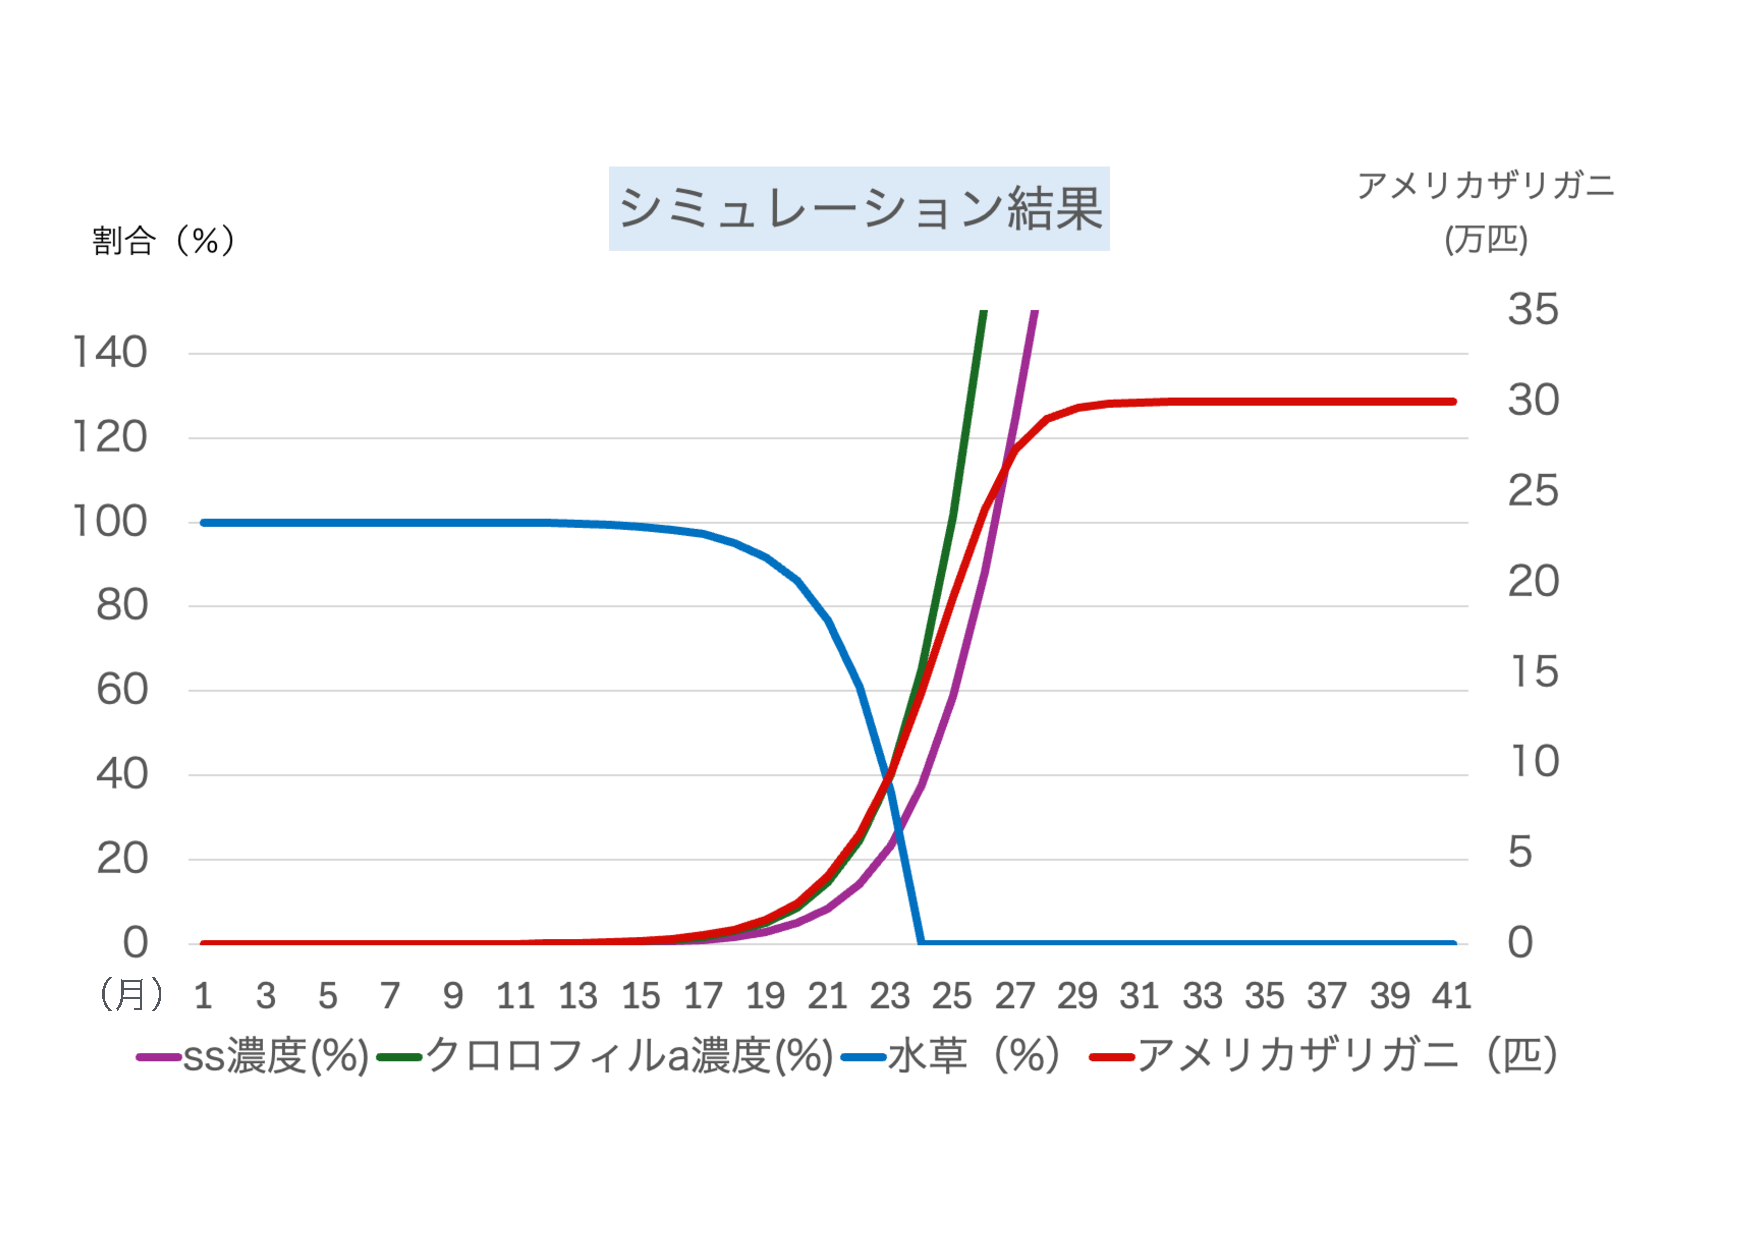
\includegraphics[width=.95\columnwidth]{graph6.pdf}
 \end{center}
 \end{figure}
\clearpage
\section{結言}

\clearpage

\section{謝辞}
本研究の遂行及び本論文の作成にあたり,須田研究室の仲間に多くの手助けを頂きました,深
く感謝の意を表します.そして,本論文の作成にあたり多大なる御指導及び御助言を頂きました,
須田宇宙准教授に深く感謝の意を表します.

\clearpage

%参考文献
\begin{thebibliography}{99}
\bibitem{FreshWater}IUCN: ``Freshwater fish highlight escalating climate impacts on species - IUCN Red List | International Union for Conservation of Nature – United States'', 
\url{https://iucnus.org/news/freshwater-fish-highlight-escalating-climate-impacts-on-species-iucn-red-list/}, (2024/09/01参照)

\bibitem{env} 環境省: ``自然環境・生物多様性'', 
\url{https://www.env.go.jp/nature/amezari_keii.html}, (2024/09/01参照)

\bibitem{nani} 環境省: ``何が問題なの? 水草、全部切る!?'', 
\url{https://www.env.go.jp/nature/amezari_mondai.html}, (2024/09/01参照)

\bibitem{log} Lotka AJ 1925 Elements of Physical Biology (Baltimore, MD Williams Wilkins Co.)
\end{thebibliography}                      

\end{document}